\begin{figure*}
  \centering

  % Define block styles used later

  \tikzstyle{module}=[draw, draw=blue!80, text width=10em, 
  text centered, minimum height=5em, minimum width = 15em, drop shadow, rounded corners,
  fill=blue!30]
  
  \tikzstyle{vecArrow} = [thick, decoration={markings,mark=at position
    1 with {\arrow[semithick]{open triangle 60}}},
  double distance=1.4pt, shorten >= 5.5pt,
  preaction = {decorate},
  postaction = {draw,line width=1.4pt, white,shorten >= 4.5pt}]

  % Define distances for bordering
  \def\blockdist{1.5}
  \def\edgedist{2.5}

  \begin{tikzpicture}[node distance=3cm,thick,scale=0.6, every node/.style={scale=0.6},path image/.style={
      path picture={
        \node at (path picture bounding box.center) {
          \includegraphics[width=1cm]{#1}
        };}}]
    \tikzstyle{conefill} = [path image=,fill opacity=0.8]
    \node[module=above:pre] (pre) at (4.5,-2.6) {\Large Pre-processing};
    \node[module,below of=pre] (seg) {\Large Segmentation};
    \node[module,below of=seg] (reg) {\Large Registration};

    \path[->,dashed] (seg.west) edge [bend right=70] node {} (reg.west);
    \path[->,dashed] (reg.east) edge [bend right=70] node {} (seg.east);

    \draw[->] (pre)--(seg);
    \draw[->] (seg)--(reg);

    \begin{pgfonlayer}{background}
      \path (pre.west |- pre.north)+(-0.9,1.0+\blockdist) node (a) {};
      \path (reg.east |- reg.south)+(+0.9,-0.5) node (b) {};
      
      \path[fill=blue!10,rounded corners, draw=blue!20, dashed] (a) rectangle (b);
    \end{pgfonlayer}
    
    \path (pre.north) +(0,+\blockdist) node (bgreg) {\Large Image regularization};

    \begin{scope}[node distance=10cm]
      \node[module] (det) [below right=0cm and 3cm of pre] {\Large Features detection};
    \end{scope}
    \begin{scope}[node distance=3.5cm]
      \node[module,above of=det] (roi) {\Large ROIs\\detection/selection};
    \end{scope}
    \node[module,below of=det] (sel) {\Large Features\\selection/extraction};
    \node[module,below of=sel] (cla) {\Large Features\\classification/fusion};

    \draw[->] (roi)--(det);
    \draw[->] (det)--(sel);
    \draw[->] (sel)--(cla);

    \begin{pgfonlayer}{background}
      \path (roi.west |- roi.north)+(-0.25,0.8) node (c) {};
      \path (roi.east |- roi.south)+(+0.25,-0.25) node (d) {};
      
      \path[fill=blue!20,rounded corners, draw=blue!25, dashed] (c) rectangle (d);
    \end{pgfonlayer}

    \path (roi.west |- roi.north) +(.6,0.4) node (bgfea) {\Large \textbf{CADe}};

    \begin{pgfonlayer}{background}
      \path (det.west |- det.north)+(-0.25,0.8) node (c) {};
      \path (cla.east |- cla.south)+(+0.25,-0.25) node (d) {};
      
      \path[fill=blue!20,rounded corners, draw=blue!25, dashed] (c) rectangle (d);
    \end{pgfonlayer}

    \path (roi.west |- det.north) +(.6,0.4) node (bgfea) {\Large \textbf{CADx}};     

    % Define the place where the arrow should start anf finish
    \path (seg.east |- seg.north)+(+0.9,0) node (e) {};
    \path (sel.west |- seg.north)+(-0.8,0) node (f) {};

    \draw[double distance =3pt,preaction={-triangle 90,thin,draw,shorten >=-1mm}] (e) -- (f) node[midway,above] {\Large Regularized data};

    \begin{scope}[yshift=34,xshift=-86]
      \transparent{0.6}\draw[path image=12_figures/figures/tikzimage/t2.eps] (0,0) rectangle (1.0,1.0);
    \end{scope}

    \begin{scope}[yshift=31,xshift=-83]
      \transparent{0.6}\draw[path image=12_figures/figures/tikzimage/t2.eps] (0,0) rectangle (1.0,1.0);
    \end{scope}

    \begin{scope}[yshift=28,xshift=-80]
      \transparent{0.8}\draw[path image=12_figures/figures/tikzimage/t2.eps] (0,0) rectangle (1.0,1.0);
      \path (0,0)+(-1.5,0.3) node {\Large T$_2$-W MRI};
    \end{scope}

    \begin{scope}[yshift=-33,xshift=-86]
      \transparent{0.6}\draw[path image=12_figures/figures/tikzimage/t2.eps] (0,0) rectangle (1.0,1.0);
    \end{scope}

    \begin{scope}[yshift=-36,xshift=-83]
      \transparent{0.6}\draw[path image=12_figures/figures/tikzimage/t2.eps] (0,0) rectangle (1.0,1.0);
    \end{scope}

    \begin{scope}[yshift=-39,xshift=-80]
      \transparent{0.8}\draw[path image=12_figures/figures/tikzimage/t2.eps] (0,0) rectangle (1.0,1.0);
      \path (0,0)+(-1.2,0.3) node {\Large T$_2$ map};
    \end{scope}

    \begin{scope}[yshift=-100,xshift=-86]
      \transparent{0.6}\draw[path image=12_figures/figures/tikzimage/dce.eps] (0,0) rectangle (1.0,1.0);
    \end{scope}

    \begin{scope}[yshift=-103,xshift=-83]
      \transparent{0.6}\draw[path image=12_figures/figures/tikzimage/dce.eps] (0,0) rectangle (1.0,1.0);
    \end{scope}

    \begin{scope}[yshift=-106,xshift=-80]
      \transparent{0.8}\draw[path image=12_figures/figures/tikzimage/dce.eps] (0,0) rectangle (1.0,1.0);
      \path (0,0)+(-1.5,0.3) node {\Large DCE MRI};
    \end{scope}

    \begin{scope}[yshift=-167,xshift=-86]
      \transparent{0.6}\draw[path image=12_figures/figures/tikzimage/dwi1.eps] (0,0) rectangle (1.0,1.0);
    \end{scope}

    \begin{scope}[yshift=-170,xshift=-83]
      \transparent{0.6}\draw[path image=12_figures/figures/tikzimage/dwi1.eps] (0,0) rectangle (1.0,1.0);
    \end{scope}

    \begin{scope}[yshift=-173,xshift=-80]
      \transparent{0.8}\draw[path image=12_figures/figures/tikzimage/dwi1.eps] (0,0) rectangle (1.0,1.0);
      \path (0,0)+(-1.5,0.3) node {\Large DW MRI};
    \end{scope}

    \begin{scope}[yshift=-234,xshift=-86]
      \transparent{0.6}\draw[path image=12_figures/figures/tikzimage/adc.eps] (0,0) rectangle (1.0,1.0);
    \end{scope}

    \begin{scope}[yshift=-237,xshift=-83]
      \transparent{0.6}\draw[path image=12_figures/figures/tikzimage/adc.eps] (0,0) rectangle (1.0,1.0);
    \end{scope}

    \begin{scope}[yshift=-240,xshift=-80]
      \transparent{0.8}\draw[path image=12_figures/figures/tikzimage/adc.eps] (0,0) rectangle (1.0,1.0);
      \path (0,0)+(-1.5,0.3) node {\Large ADC};
    \end{scope}

    \begin{scope}[yshift=-301,xshift=-86]
      \transparent{0.6}\draw[path image=12_figures/figures/tikzimage/mrsi.eps] (0,0) rectangle (1.0,1.0);
    \end{scope}

    \begin{scope}[yshift=-304,xshift=-83]
      \transparent{0.6}\draw[path image=12_figures/figures/tikzimage/mrsi.eps] (0,0) rectangle (1.0,1.0);
    \end{scope}

    \begin{scope}[yshift=-307,xshift=-80]
      \transparent{0.8}\draw[path image=12_figures/figures/tikzimage/mrsi.eps] (0,0) rectangle (1.0,1.0);
      \path (0,0)+(-1,0.3) node {\Large MRSI};
    \end{scope}

    \path (pre.west |- roi.north)+(-3.5,1.0+\blockdist) node (g) {};
    \path (reg.west |- cla.south)+(-3.5,-0.5) node (h) {};

    \draw[decorate,decoration={brace,raise=6pt,amplitude=10pt}, thick]
    (g)--(h) ;
    
    \path (seg.west |- seg.north)+(-2.5,0) node (i) {};
    \path (seg.west |- seg.north)+(-0.9,0) node (j) {};
    
    \draw[double distance =3pt,preaction={-triangle 90,thin,draw,shorten >=-1mm}] (i) -- (j);   

    \path (sel.east |- seg.north)+(2,0) node (k) {};
    \path (sel.east |- seg.north)+(0.5,0) node (l) {};
    
  \end{tikzpicture}
  \caption{Common \ac{cad} framework based on \ac{mri} images used to detect \ac{cap}.}
  \label{fig:wkfcad}
\end{figure*}


\begin{figure*}
  \centering
  \hspace*{\fill}
  \subfigure[\ac{t2w}-\ac{mri} slice of an healthy prostate acquire with a 1.5 Tesla \ac{mri}. The blue contour represents the \ac{cg} while the \ac{pz} corresponds to the green contour.]{\label{subfig:t2whealthy}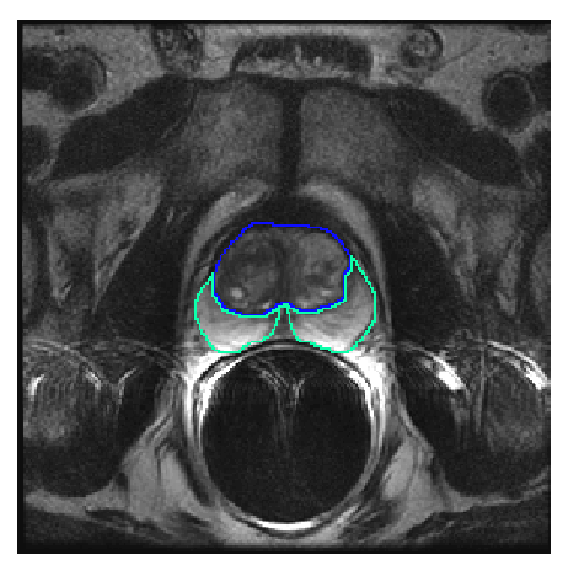
\includegraphics[width=0.3\linewidth]{12_figures/figures/t2w/t2w_healthy.eps}} \hfill
  \subfigure[\ac{t2w}-\ac{mri} slice of a prostate with a \ac{cap} highlighted in the \ac{pz} using a 3.0 Tesla \ac{mri} scanner.]{\label{subfig:t2wcancerpz}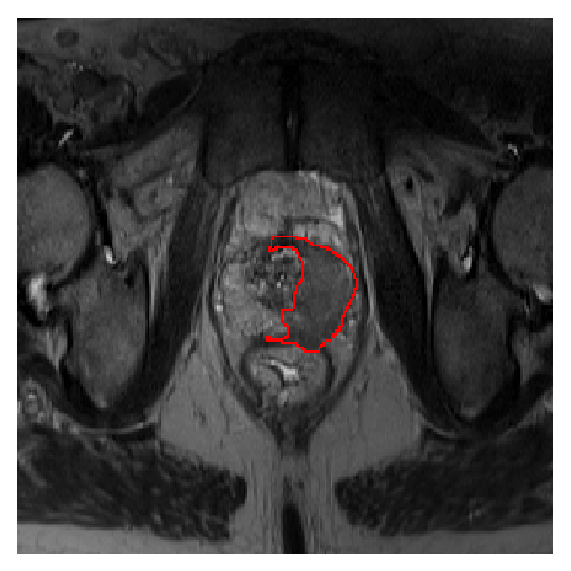
\includegraphics[width=0.3\linewidth]{12_figures/figures/t2w/t2w_cancer_pz.eps}} \hfill
  \subfigure[\ac{t2w}-\ac{mri} slice of a prostate with a \ac{cap} highlighted in the \ac{cg} using a 3.0 Tesla \ac{mri} scanner.]{\label{subfig:t2wcancercg}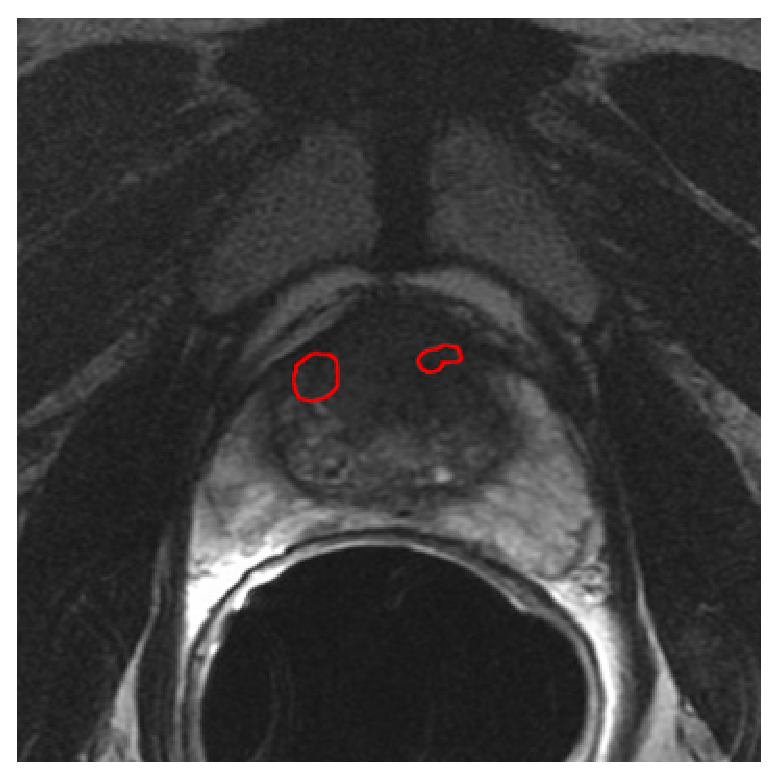
\includegraphics[width=0.3\linewidth]{12_figures/figures/t2w/t2w_cancer_cg.eps}}
  \hspace*{\fill}
  \caption{Rendering of \ac{t2w}-\ac{mri} prostate image with both 1.5 and 3.0 Tesla \ac{mri} scanner.}
  \label{fig:t2w}
\end{figure*}


\begin{figure*}
  \centering
  \hspace*{\fill}
  \subfigure[\ac{t1w}-\ac{mri} image where the cancer is delimited by the red contour. The green area was still not invaded by the \ac{cap}]{\label{subfig:t1w}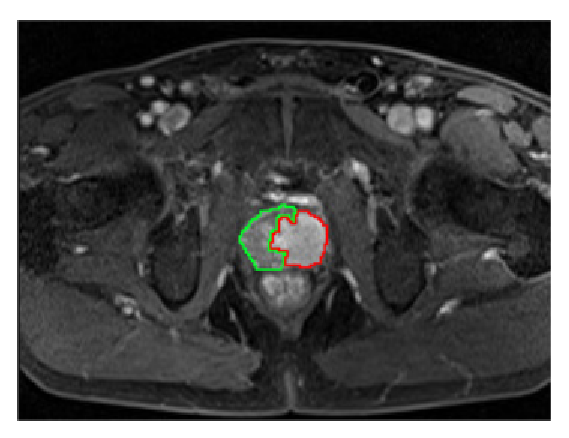
\includegraphics[width=0.4\linewidth]{12_figures/figures/dce/slice.eps}} \hfill
  \subfigure[Enhancement curve computed during the \ac{dce}-\ac{mri} analysis. The red curve is typical from \ac{cap} cancer while the green curve is characteristic of healthy tissue.]{\label{subfig:dce}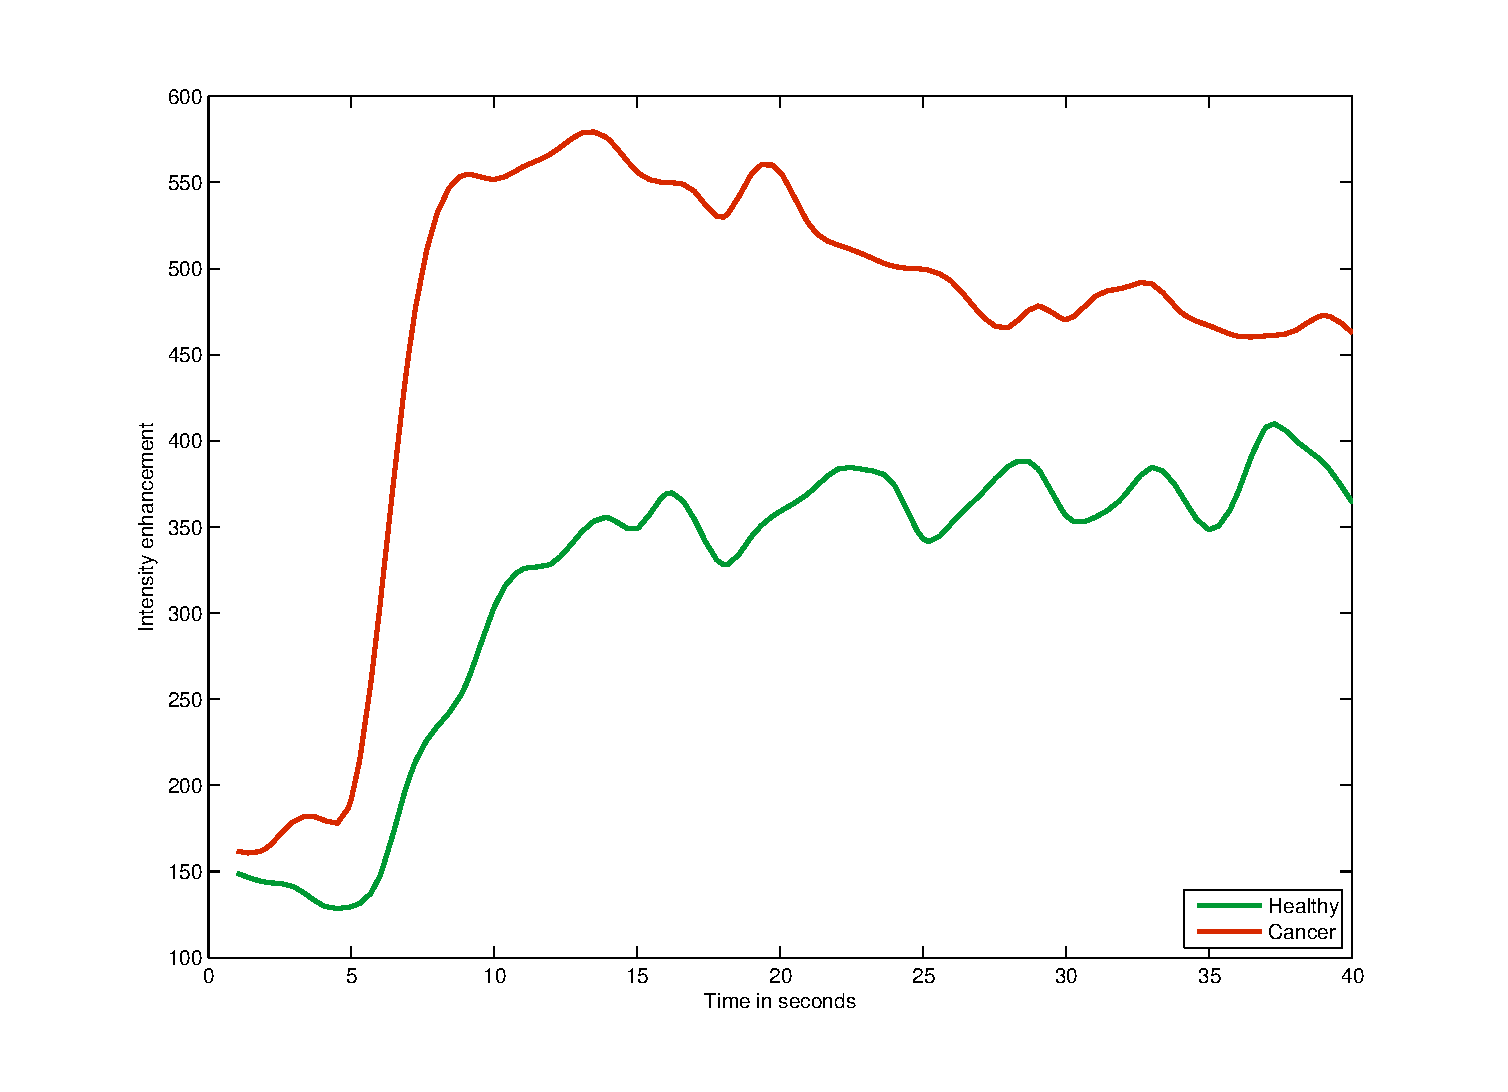
\includegraphics[width=0.45\linewidth]{12_figures/figures/dce/dce_cancer_healthy.eps}}
  \hspace*{\fill}
  \caption{Illustration of typical enhancement signal observed in \ac{dce}-\ac{mri} analysis collected with a 3.0 Tesla \ac{mri} scanner.}
  \label{fig:dceana}
\end{figure*}


\begin{figure}
  \centering
  \hspace*{\fill}
  \subfigure[\ac{dw}-\ac{mri} image. The cancer corresponds to the high \ac{si} region highlighted in red.]{\label{subfig:dwi}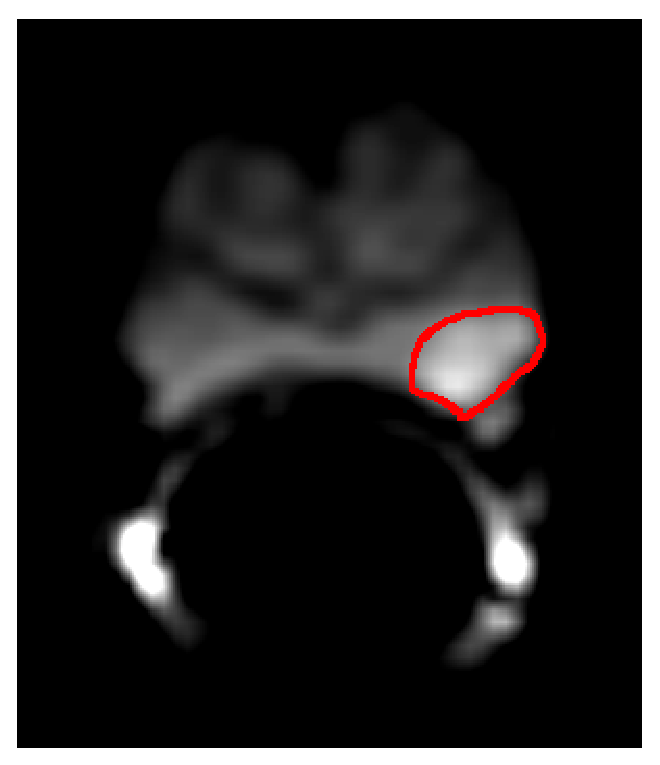
\includegraphics[height=0.2\textheight]{12_figures/figures/dwi/dwi_cancer.eps}} \hfill
  \subfigure[\ac{adc} map computer. The cancer corresponds to the low \ac{si} region highlighted in red.]{\label{subfig:adc}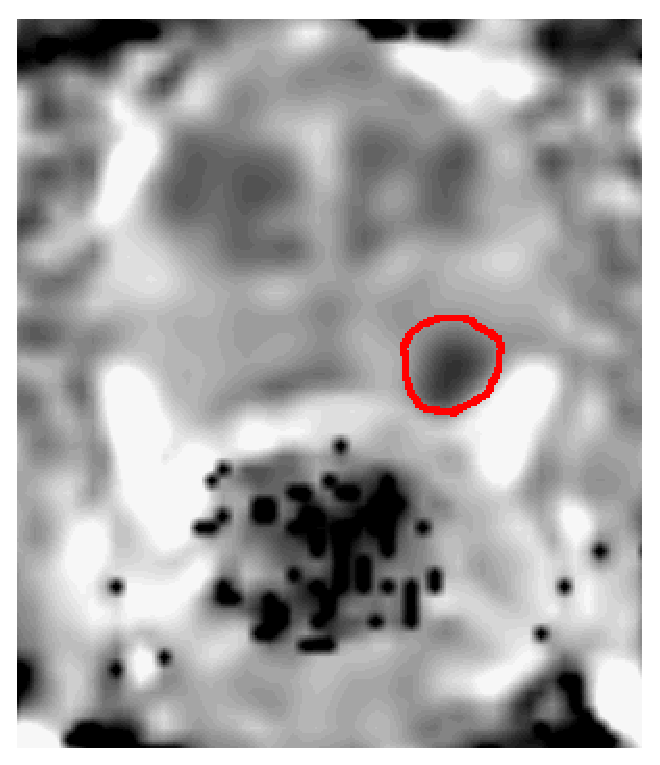
\includegraphics[height=0.2\textheight]{12_figures/figures/dwi/adc_cancer.eps}}
  \hspace*{\fill}
  \caption{Illustration of of \ac{dw}-\ac{mri} and \ac{adc} map. The signal intensity corresponding to cancer are inversely correlated on these two types of imaging techniques.}
  \label{fig:dwi}
\end{figure}


\begin{figure*}
  \centering
  \hspace*{\fill}
  \subfigure[]{\label{subfig:mrsihea}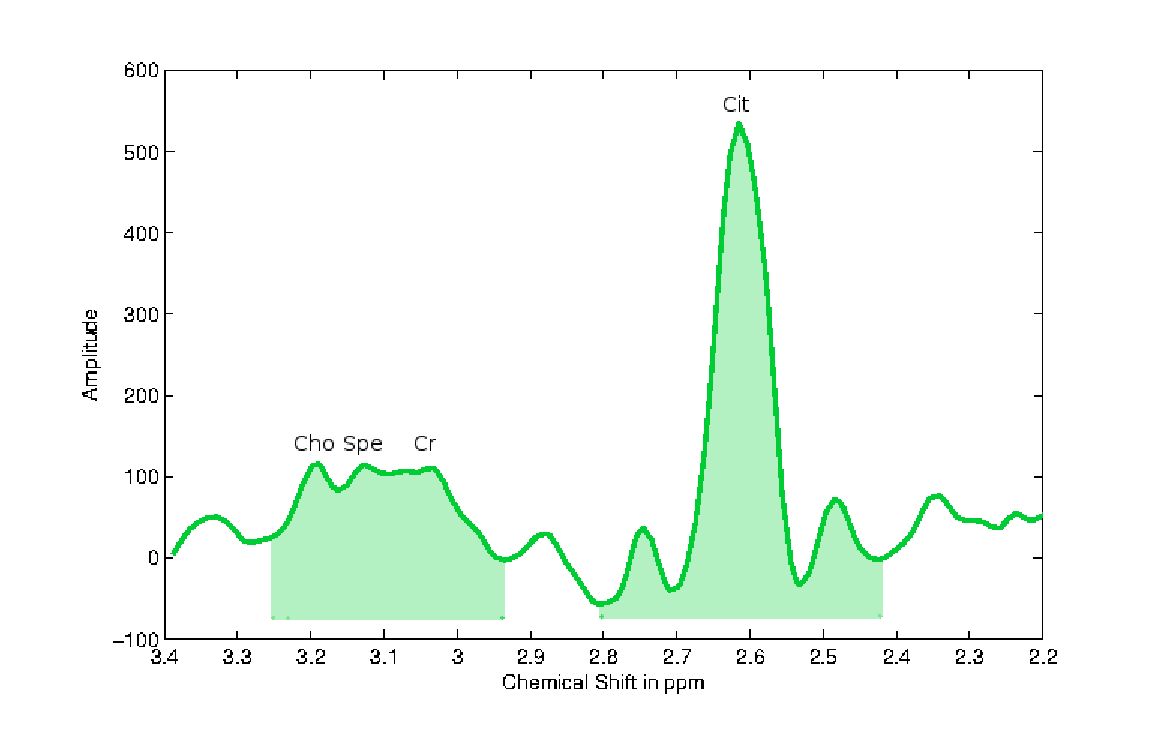
\includegraphics[width=0.45\linewidth]{12_figures/figures/mrsi/mrsi_healthy.eps}} \hfill
  \subfigure[]{\label{subfig:mrsican}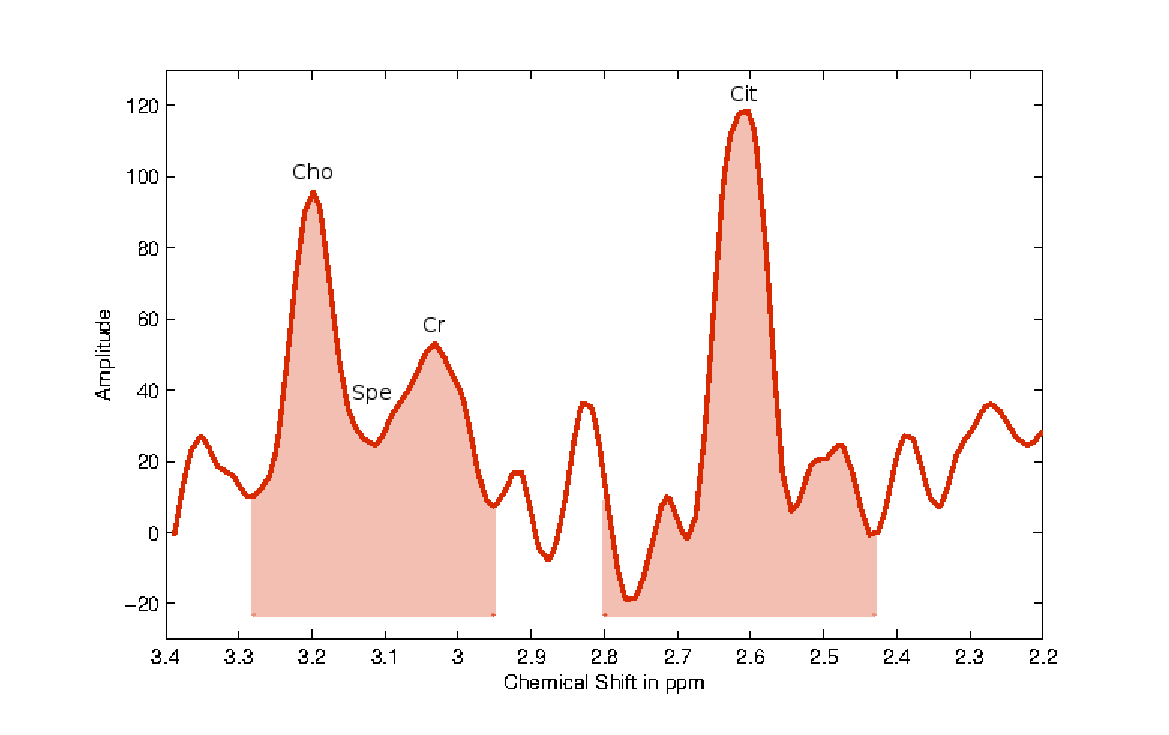
\includegraphics[width=0.45\linewidth]{12_figures/figures/mrsi/mrsi_cancer.eps}}
  \hspace*{\fill}
  \caption{Illustration of an \ac{mrsi} spectrum both healthy (Fig. \ref{subfig:mrsihea}) and cancerous (Fig. \ref{subfig:mrsican}) voxel with a 3.0 Tesla \ac{mri}. The highlighted areas corresponds to the related concentration of the metabolites which is computed by integrating the area under each peak. Acronyms: Choline (Cho), Spermine (Spe), Creatine (Cr) and Citrate (Cit).}
  \label{fig:mrsi}
\end{figure*}

\begin{figure}
  \centering
  \hspace*{\fill}
  \subfigure[Illustration and location of the bladder on a \ac{t2w}-\ac{mri} image acquired with a 3.0 Tesla \ac{mri} scanner]{\label{subfig:bladder} 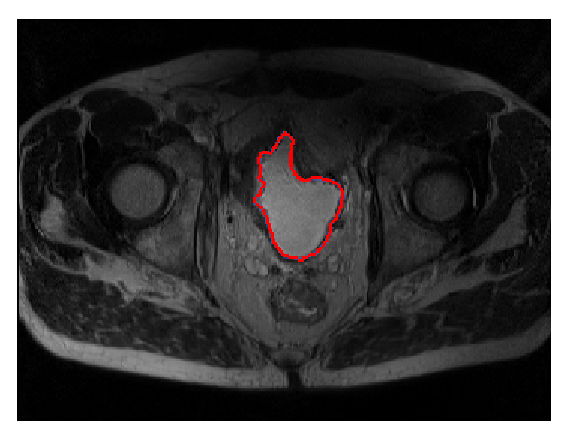
\includegraphics[width=0.4\linewidth]{12_figures/figures/niaf/t2w_bladder.eps}} \hfill
  \subfigure[Illustration and location of the femoral arteries on a \ac{t1w}-\ac{mri} image acquired with a 3.0 Tesla \ac{mri} scanner]{\label{subfig:arteries} 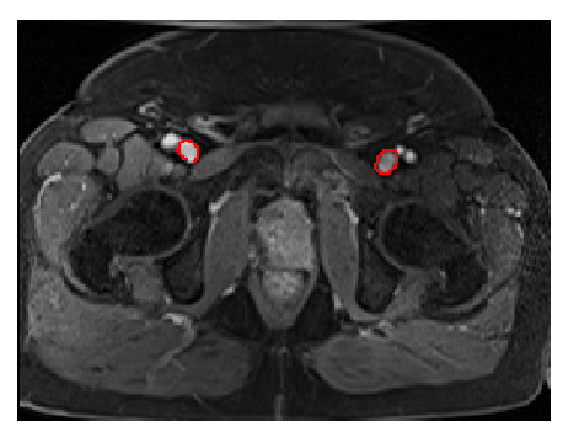
\includegraphics[width=0.4\linewidth]{12_figures/figures/niaf/t1w_arteries.eps}}
  \hspace*{\fill}
  \caption{Illustration of the two organs used by \cite{Niaf2011,Niaf2012} to normalize \ac{t2w} and \ac{t1w} \ac{mri} images.}
  \label{fig:niaf}
\end{figure}

\begin{figure}
  \centering
  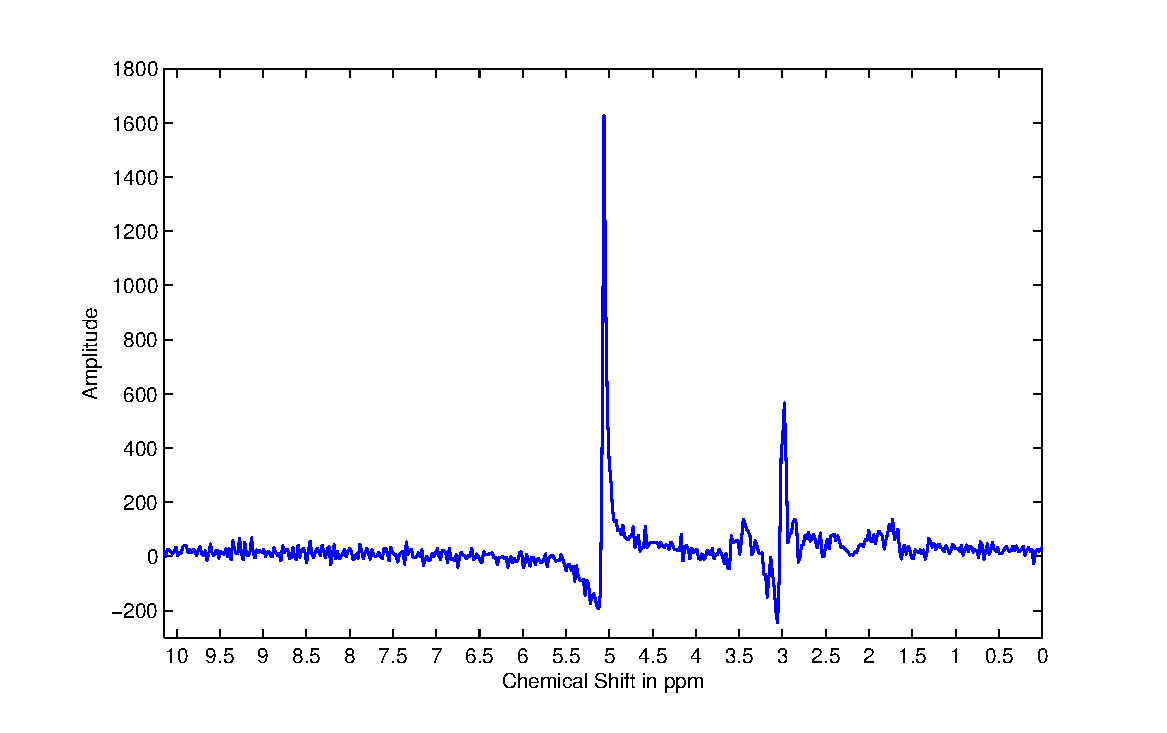
\includegraphics[width=0.6\linewidth]{12_figures/figures/phase/phase.eps}
  \caption{Illustration of frequency and phase misalignment in an \ac{mrsi} spectra acquired with a 3.0 Tesla \ac{mrsi} scanner. Focusing on the phase misalignment, note the distortion of the signal specially visible for the water (cf., around 5.1 ppm) and citrate (cf., around 3 ppm) peaks. Regarding the frequency misalignment, the water peak is known to be aligned at 4.65 ppm. However, it can observed that this peak is occurring around 5.1 ppm.}
  \label{fig:phase}
\end{figure}

\begin{figure}
  \centering
  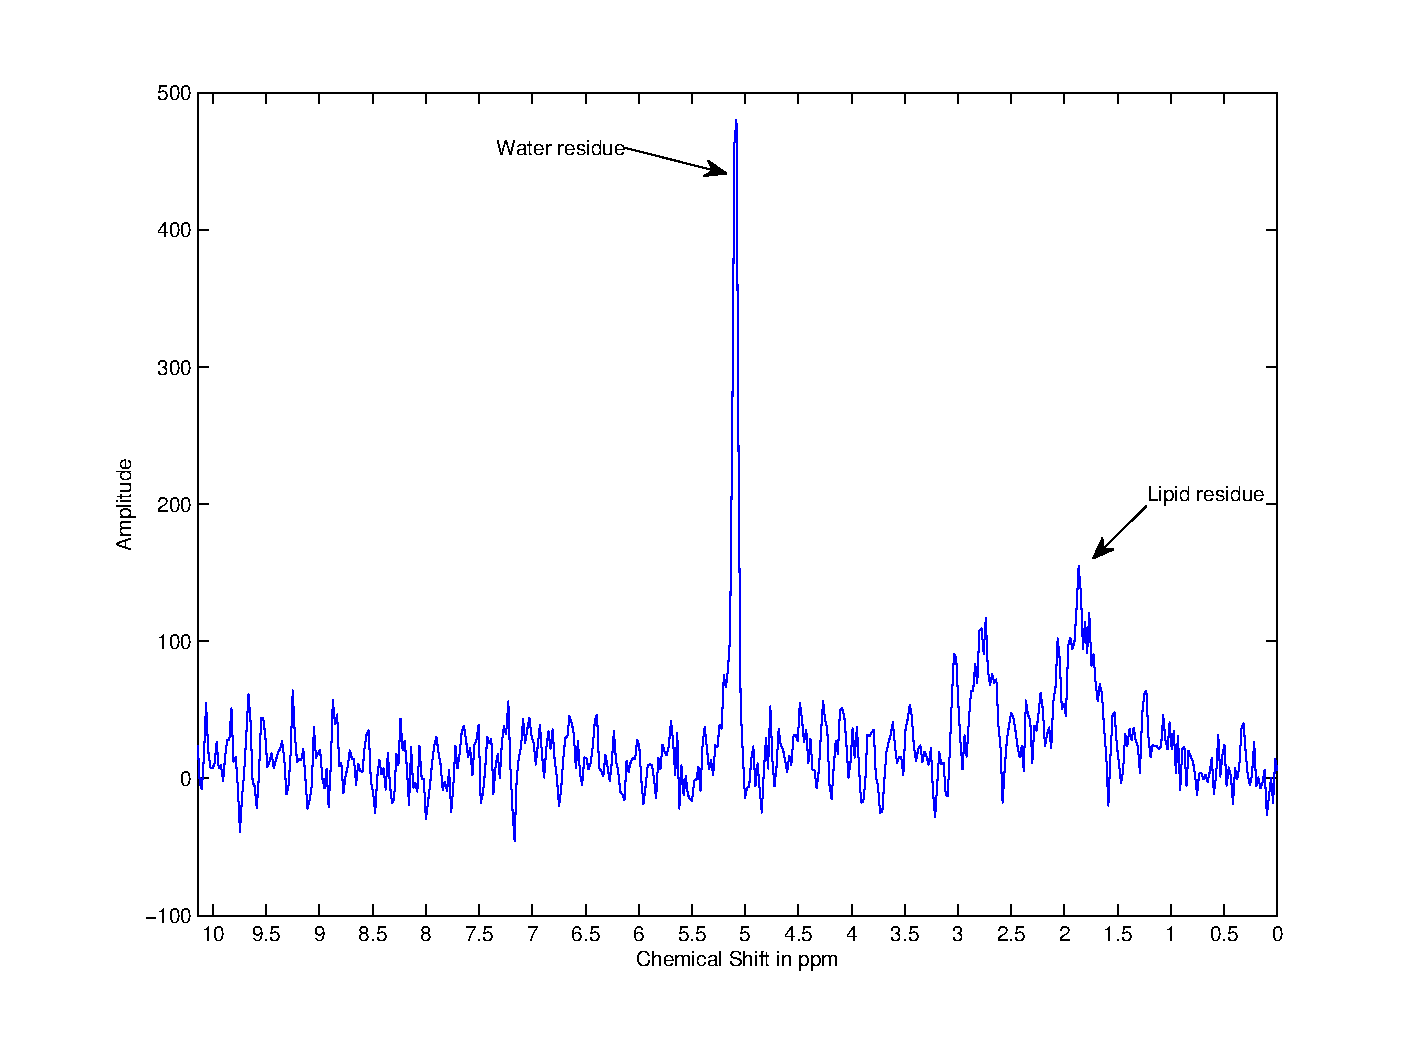
\includegraphics[width=0.6\linewidth]{12_figures/figures/water/water_fat.eps}
  \caption{Illustration of the residues of water and fat even after their suppression during the acquisition protocol. The acquisition was carried out with a 3.0 Tesla \ac{mri}.}
  \label{fig:waterfat}
\end{figure}

\begin{figure}
  \centering

  % Define block styles used later

  \tikzstyle{module}=[draw, draw=blue!80, text width=10em, 
  text centered, minimum height=5em, minimum width = 10em, drop shadow, rounded corners,
  fill=blue!30]
  
  \tikzstyle{vecArrow} = [thick, decoration={markings,mark=at position
    1 with {\arrow[semithick]{open triangle 60}}},
  double distance=1.4pt, shorten >= 5.5pt,
  preaction = {decorate},
  postaction = {draw,line width=1.4pt, white,shorten >= 4.5pt}]

  % Define distances for bordering
  \def\blockdist{1.5}
  \def\edgedist{2.5}

  \definecolor{darkblue}{rgb}{0.2,0.2,0.6}
  \definecolor{darkred}{rgb}{0.6,0.1,0.1}
  \definecolor{darkgreen}{rgb}{0.2,0.6,0.2}

  \def\arrow{
    (10.75:1.1) -- (6.5:1) arc (6.25:120:1) [rounded corners=0.5] --
    (120:0.9) [rounded corners=1] -- (130:1.1) [rounded corners=0.5] --
    (120:1.3) [sharp corners] -- (120:1.2) arc (120:5.25:1.2)
    [rounded corners=1] -- (10.75:1.1) -- (6.5:1) -- cycle
  }

  \tikzset{
    ashadow/.style={opacity=.25, shadow xshift=0.07, shadow yshift=-0.07},
  }

  \def\arrows[#1]{         
    \begin{scope}[scale=#1]
      \node[align=center] at (0,0) {\Huge{ Loop } \\ \Huge{ until matching } };  
      
      \draw[color=darkred, %
      drop shadow={ashadow, color=red!60!black}] \arrow;

      \draw[color=darkgreen, bottom color=green!60!black, top color=green!30, %
      drop shadow={ashadow, color=green!60!black}] [rotate=120] \arrow;

      \draw[color=darkblue, right color=blue!60, left color=blue!30, %
      drop shadow={ashadow, color=blue!60!black}] [rotate=240] \arrow;

      % to hide the green shadow
      \draw[color=darkred, left color=red!60, right color=red!30] \arrow;
    \end{scope}
  }

  \begin{tikzpicture}[node distance=3cm,thick,scale=0.5, every node/.style={scale=0.5},path image/.style={
      path picture={
        \node at (path picture bounding box.center) {
          \includegraphics[width=1cm]{#1}
        };}}]
    \tikzstyle{conefill} = [path image=,fill opacity=0.8]

    \node (t2w) at (0,0)	{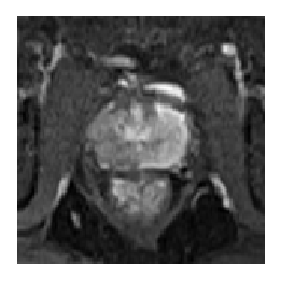
\includegraphics[width=1.5cm]{12_figures/figures/tikzimage/dce.eps}};
    \begin{scope}[node distance=1.2cm]
      \node[below of=t2w] (cap1) {\Large Fixed};
    \end{scope}
    \begin{scope}[node distance=6cm]
      \node[below of=t2w] 	(dce) 			{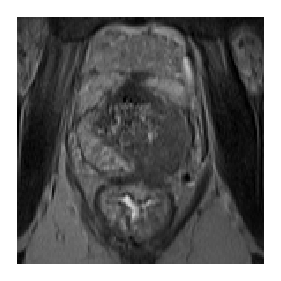
\includegraphics[width=1.5cm]{12_figures/figures/tikzimage/t2.eps}};
      \begin{scope}[node distance=1.2cm]
        \node[below of=dce] (cap2) {\Large Moving};
      \end{scope}
    \end{scope}

    \begin{scope}[node distance=5.5cm]
      \node[module,right of=t2w] (sim) {\Large Similarity \\ measure};
    \end{scope}
    \begin{scope}[node distance=3cm]
      \node[module,below of=sim] (int) {\Large Interpolator};
      \node[module,below of=int] (tra) {\Large Transform};
    \end{scope}

    \draw[line width=1mm,draw=blue!30,->] (t2w)--(sim);  
    \draw[line width=1mm,draw=blue!30,->] (dce)--(tra); 

    \begin{scope}[node distance=9cm]
      \node[module,right of=sim] (opt) {\Large Optimizer};
    \end{scope}

    \draw[draw=blue,->,line width=.5mm] (tra)--(int);
    \draw[draw=blue,->,line width=.5mm] (int)--(sim);
    \draw[draw=blue,->,line width=.5mm] (sim)--(opt) node[midway,above] {\Large Similarity} node[midway,below] {\Large metric};
    \draw[draw=blue,->,line width=.5mm] (opt)|-(tra); 

    \begin{pgfonlayer}{background}
      \path (sim.west |- sim.north)+(-0.5,.5) node (a) {};
      \path (opt.east |- tra.south)+(+0.5,-0.5) node (b) {};
      
      \path[fill=blue!10,rounded corners, draw=blue!20, dashed] (a) rectangle (b);
    \end{pgfonlayer} 

    \begin{scope}[node distance=5cm]
      \node[right of=int] (arr) {
        \begin{tikzpicture}
          \arrows[1.9];
        \end{tikzpicture}
      };
    \end{scope}
  \end{tikzpicture}
  \caption{Typical framework involved to solve the registration problem.}
  \label{fig:frareg}
\end{figure}


\begin{figure}
  \centering
  \hspace*{\fill}
  \subfigure[]{\label{subfig:histoalgn} 
\includegraphics[width=0.2\textwidth]{12_figures/figures/histogram/jointhistoalg.eps}} \hfill
  \subfigure[]{\label{subfig:histomisalgn} 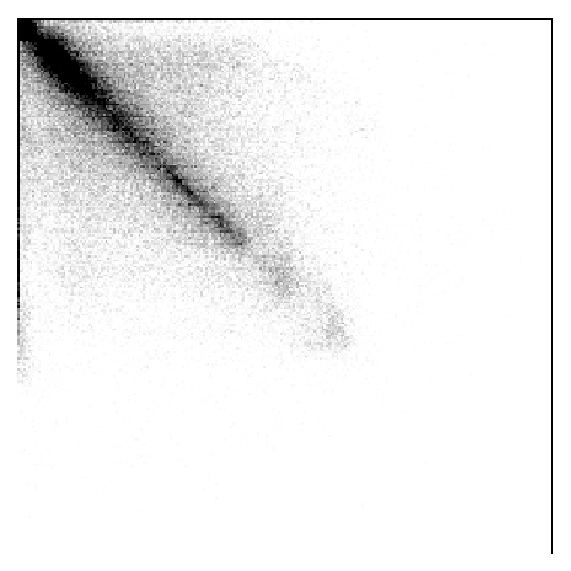
\includegraphics[width=0.2\textwidth]{12_figures/figures/histogram/jointhistomisal.eps}}
  \hspace*{\fill}
  \caption{Difference observed in joint histogram between aligned (Fig. \ref{subfig:histoalgn}) and misaligned (Fig. \ref{subfig:histomisalgn}) images.}
  \label{fig:jointhisto}
\end{figure}

\begin{figure}
  \centering
  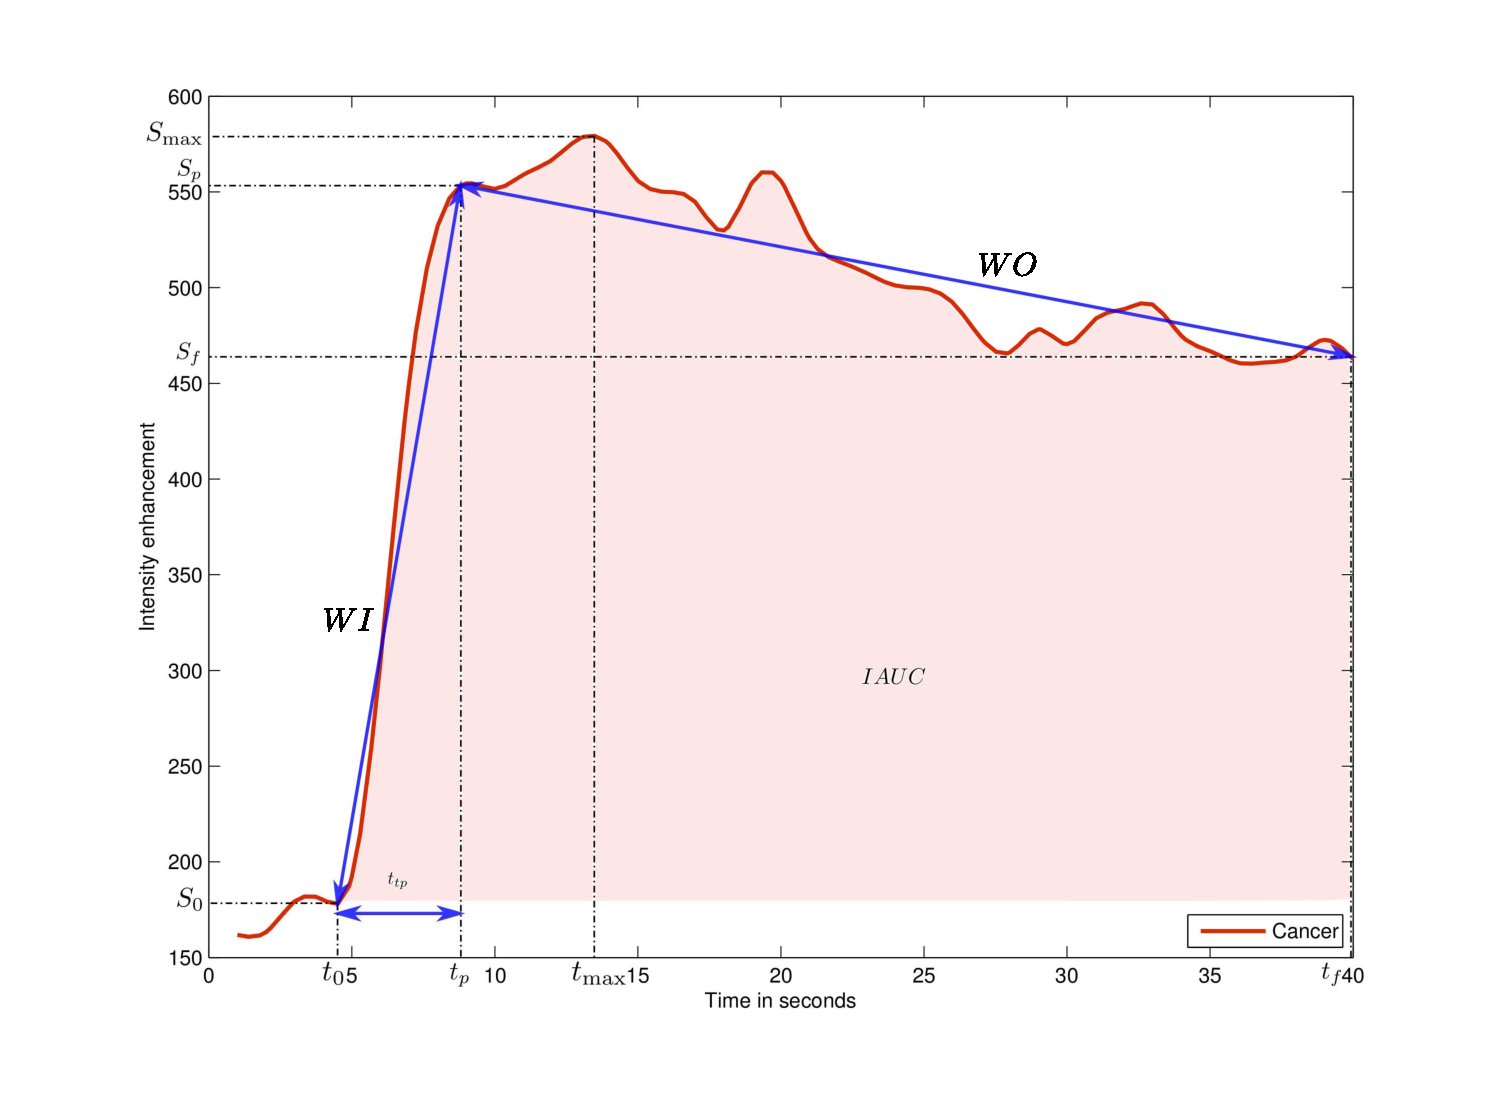
\includegraphics[width=.6\linewidth]{04_data_classification/06_feature_detection/figures/dce/dce_cancer_parameters.eps}
  \caption{Graphical representation of the different semi-quantitative features used for \ac{dce}-\ac{mri} analysis.}
  \label{fig:dceparam}
\end{figure}

\begin{figure*}
  \centering
  \hspace*{\fill}
  \subfigure[Comparison in terms of \ac{auc}-\ac{roc} of the methods using data from 1.5 Tesla \ac{mri} scanner.]{
    \label{fig:auc15}
    \begin{tikzpicture}[scale=.5,every node/.style={scale=0.5}]

      \def\labels{
        {\color{semiAuto}[2]},
        {\color{semiAuto}[3]},
        {\color{semiAuto}[6]},
        {\color{semiAuto}[7]},
        {\color{semiAuto}[9]},
        {\color{semiAuto}[15]},
        {\color{semiAuto}[16]},
        {\color{semiAuto}[19]},
        {\color{semiAuto}[20]},
        {\color{semiAuto}[30]},
        {\color{semiAuto}[31]},
        {\color{semiAuto}[32]},
        {\color{semiAuto}[33]},
        {\color{semiAuto}[39]},
        {\color{semiAuto}[41]},
        {\color{semiAuto}[18]},
        {\color{semiAuto}[25]},
        {\color{semiAuto}[40]}
      }

      \def\reward{90,94,84,87,71,93,97,87,87,84,91,90,85,91,97,92,77,90}
      \def\dbSize{25,53,15,10,25,27,55,23,30,15,19,36,29,29,29,29,100,10}
      \def\dbClass{1,2,1,1,1,1,2,1,1,1,1,1,1,1,1,1,3,1}		
      \def\cZoom{3} 
      \def\percentageLabelAngle{90}
      \def\nbeams{18}
      \pgfmathsetmacro\beamAngle{(360/\nbeams)}
      \pgfmathsetmacro\halfAngle{(180/\nbeams)}
      \pgfmathsetmacro\globalRotation{\halfAngle}

      % draw the radiants
      \foreach \n  [count=\ni] in \labels
      {
        \pgfmathsetmacro\cAngle{{(\ni*(360/\nbeams))+\globalRotation}}
        \draw	(\cAngle:{\cZoom*1.15})  node[fill=white] {\n};
        \draw [thin] (0,0) -- (\cAngle:{\cZoom*1}) ;

      }

      % draw the % rings 
      \foreach \x in {12.5,25, ...,100} 
      \draw [thin,color=gray!50] (0,0) circle [radius={\cZoom*\x/100}];

      \foreach \x in {50,75,100}
      { 
        \draw [thin,color=black!50] (0,0) circle [radius={\cZoom/100*\x}];
        \foreach \a in {0, 180} \draw ({\percentageLabelAngle+\a}:{\cZoom*0.01*\x}) node  [inner sep=0pt,outer sep=0pt,fill=white,font=\fontsize{8}{8.5}\selectfont]{$\x\%$};
      }

      % draw the path of the percentages
      \def\aux{{\reward}}
      \pgfmathsetmacro\origin{\aux[\nbeams-1]} 
      \draw [blue, thick] (\globalRotation:{\cZoom*\origin/100}) \foreach \n  [count=\ni] in \reward { -- ({(\ni*(360/\nbeams))+\globalRotation}:{\cZoom*\n/100}) } ;

      % label all the percentags
      \foreach \n [count=\ni] in \dbSize 
      {
	\pgfmathsetmacro\cAngle{{(\ni*(360/\nbeams))+\globalRotation}}
	\pgfmathsetmacro\nreward{\aux[\ni-1]}
	\draw (\cAngle:{\cZoom*1.4}) node[align=center] {{\color{blue}\nreward $\%$} \\ {\color{red}\n} };
      } ;

      % draw the database rose
      \def\dbScale{\9}
      \foreach \n [count=\ni] in \dbClass
      \filldraw[fill=red!20!white, draw=red!50!black]
      (0,0) -- ({\ni*(360/\nbeams)-\halfAngle+\globalRotation}:{\cZoom*\n/9}) arc ({\ni*(360/\nbeams)-\halfAngle+\globalRotation}:{\ni*(360/\nbeams)+\halfAngle+\globalRotation}:{\cZoom*\n/9}) -- cycle;
      \foreach \x in {1,2,3}
      \draw [thin,color=red!50!black,dashed] (0,0) circle [radius={\cZoom*\x/9}];

      %% draw the domain of each class 
      \def\puta{	15/0/{Multiparametric},
        3/15/{Monoparametric}}

      \foreach \numElm/\contadorQueNoSeCalcular/\name [count=\ni] in \puta
      {

 	\pgfmathsetmacro\initialAngle{(\contadorQueNoSeCalcular*\beamAngle)+\halfAngle+\globalRotation}
 	\pgfmathsetmacro\finalAngle  {((\numElm+\contadorQueNoSeCalcular)*\beamAngle)+\halfAngle+\globalRotation}
	\pgfmathsetmacro\l  {\cZoom*1.5+.3pt}
	\draw (\initialAngle:{\cZoom*1.6}) -- (\initialAngle:{\cZoom*1.1});
	\draw [ |<->|,>=latex] (\initialAngle:\l) arc (\initialAngle:\finalAngle:\l) ;    									 
	\pgfmathsetmacro\r  {\cZoom*1.5+.45pt}
    	{\draw [decoration={raise=4pt,text along path,text={\name},text align={center}},decorate] (\finalAngle:\r) arc (\finalAngle:\initialAngle:\r);}
      }
      
    \end{tikzpicture}}\hfill
  \subfigure[Comparison in terms of \ac{auc}-\ac{roc} of the methods using data from 3.0 Tesla \ac{mri} scanner.]{
    \label{fig:auc30}
    \begin{tikzpicture}[scale=.5,every node/.style={scale=0.5}]

      \def\labels{
        {\color{semiAuto}[12]},
        {\color{semiAuto}[14]},
        {\color{semiAuto}[24]},
        {\color{semiAuto}[36]},
        {\color{semiAuto}[37]},
        {\color{semiAuto}[38]}
      }

      \def\reward{81,83,95,82,77,80}
      \def\dbSize{347,54,48,6,12,22}
      \def\dbClass{3,3,2,1,1,1}		
      \def\cZoom{3} 
      \def\percentageLabelAngle{90}
      \def\nbeams{6}
      \pgfmathsetmacro\beamAngle{(360/\nbeams)}
      \pgfmathsetmacro\halfAngle{(180/\nbeams)}
      \pgfmathsetmacro\globalRotation{\halfAngle}

      % draw the radiants
      \foreach \n  [count=\ni] in \labels
      {
        \pgfmathsetmacro\cAngle{{(\ni*(360/\nbeams))+\globalRotation}}
        \draw	(\cAngle:{\cZoom*1.15})  node[fill=white] {\n};
        \draw [thin] (0,0) -- (\cAngle:{\cZoom*1}) ;

      }

      % draw the % rings 
      \foreach \x in {12.5,25, ...,100} 
      \draw [thin,color=gray!50] (0,0) circle [radius={\cZoom*\x/100}];

      \foreach \x in {50,75,100}
      { 
        \draw [thin,color=black!50] (0,0) circle [radius={\cZoom/100*\x}];
        \foreach \a in {0, 180} \draw ({\percentageLabelAngle+\a}:{\cZoom*0.01*\x}) node  [inner sep=0pt,outer sep=0pt,fill=white,font=\fontsize{8}{8.5}\selectfont]{$\x\%$};
      }

      % draw the path of the percentages
      \def\aux{{\reward}}
      \pgfmathsetmacro\origin{\aux[\nbeams-1]} 
      \draw [blue, thick] (\globalRotation:{\cZoom*\origin/100}) \foreach \n  [count=\ni] in \reward { -- ({(\ni*(360/\nbeams))+\globalRotation}:{\cZoom*\n/100}) } ;

      % label all the percentags
      \foreach \n [count=\ni] in \dbSize 
      {
	\pgfmathsetmacro\cAngle{{(\ni*(360/\nbeams))+\globalRotation}}
	\pgfmathsetmacro\nreward{\aux[\ni-1]}
	\draw (\cAngle:{\cZoom*1.4}) node[align=center] {{\color{blue}\nreward $\%$} \\ {\color{red}\n} };
      } ;

      % draw the database rose
      \def\dbScale{\9}
      \foreach \n [count=\ni] in \dbClass
      \filldraw[fill=red!20!white, draw=red!50!black]
      (0,0) -- ({\ni*(360/\nbeams)-\halfAngle+\globalRotation}:{\cZoom*\n/9}) arc ({\ni*(360/\nbeams)-\halfAngle+\globalRotation}:{\ni*(360/\nbeams)+\halfAngle+\globalRotation}:{\cZoom*\n/9}) -- cycle;
      \foreach \x in {1,2,3}
      \draw [thin,color=red!50!black,dashed] (0,0) circle [radius={\cZoom*\x/9}];

      %% draw the domain of each class 
      \def\puta{	5/0/{Multiparametric},
        1/5/{Monoparametric}}

      \foreach \numElm/\contadorQueNoSeCalcular/\name [count=\ni] in \puta
      {

 	\pgfmathsetmacro\initialAngle{(\contadorQueNoSeCalcular*\beamAngle)+\halfAngle+\globalRotation}
 	\pgfmathsetmacro\finalAngle  {((\numElm+\contadorQueNoSeCalcular)*\beamAngle)+\halfAngle+\globalRotation}
	\pgfmathsetmacro\l  {\cZoom*1.5+.3pt}
	\draw (\initialAngle:{\cZoom*1.6}) -- (\initialAngle:{\cZoom*1.1});
	\draw [ |<->|,>=latex] (\initialAngle:\l) arc (\initialAngle:\finalAngle:\l) ;    									 
	\pgfmathsetmacro\r  {\cZoom*1.5+.45pt}
    	{\draw [decoration={raise=4pt,text along path,  text={\name},text align={center}},decorate] (\finalAngle:\r) arc (\finalAngle:\initialAngle:\r);}
      }
      
    \end{tikzpicture}
  }
  \hspace*{\fill}
  \caption{Comparison of the results in terms of AUC for 1.5 and 3.0 Tesla \ac{mri} scanners. The {\color{blue}blue} value represents the metric and are graphically reported in the blue curve in the center of the figure. The {\color{red}red} value and areas correspond to the number of patients in the dataset. The numbers between brackets in {\color{semiAuto}green} correspond to the reference as reported in Tab. \ref{tab:sumpap}.}
  \label{fig:auc}
\end{figure*}

% ------------------------------------------------------------------------------------------------------------------------

\begin{figure*}%
  \centering
  \hspace*{\fill}
  \subfigure[Comparison in terms of sensitivity of the methods using data from 1.5 Tesla \ac{mri} scanner.]{
    \label{fig:sens15}
    \begin{tikzpicture}[scale=.5,every node/.style={scale=0.5}]

      \def\labels{
        {\color{semiAuto}[4]},
        {\color{semiAuto}[5]},
        {\color{semiAuto}[7]},
        {\color{semiAuto}[13]},
        {\color{semiAuto}[15]},
        {\color{semiAuto}[21]},
        {\color{semiAuto}[22]},
        {\color{semiAuto}[29]},
        {\color{semiAuto}[34]},
        {\color{semiAuto}[18]},
        {\color{semiAuto}[25]},
        {\color{semiAuto}[28]}
      }

      \def\reward{74,66,79,90,85,76,78,84,88,82,100,87}
      \def\dbSize{10,21,10,11,27,20,20,18,16,10,100,18}
      \def\dbClass{1,2,1,1,2,1,1,1,1,1,3,1}		
      \def\cZoom{3} 
      \def\percentageLabelAngle{90}
      \def\nbeams{12}
      \pgfmathsetmacro\beamAngle{(360/\nbeams)}
      \pgfmathsetmacro\halfAngle{(180/\nbeams)}
      \pgfmathsetmacro\globalRotation{\halfAngle}

      % draw the radiants
      \foreach \n  [count=\ni] in \labels
      {
        \pgfmathsetmacro\cAngle{{(\ni*(360/\nbeams))+\globalRotation}}
        \draw	(\cAngle:{\cZoom*1.15})  node[fill=white] {\n};
        \draw [thin] (0,0) -- (\cAngle:{\cZoom*1}) ;

      }

      % draw the % rings 
      \foreach \x in {12.5,25, ...,100} 
      \draw [thin,color=gray!50] (0,0) circle [radius={\cZoom*\x/100}];

      \foreach \x in {50,75,100}
      { 
        \draw [thin,color=black!50] (0,0) circle [radius={\cZoom/100*\x}];
        \foreach \a in {0, 180} \draw ({\percentageLabelAngle+\a}:{\cZoom*0.01*\x}) node  [inner sep=0pt,outer sep=0pt,fill=white,font=\fontsize{8}{8.5}\selectfont]{$\x\%$};
      }

      % draw the path of the percentages
      \def\aux{{\reward}}
      \pgfmathsetmacro\origin{\aux[\nbeams-1]} 
      \draw [blue, thick] (\globalRotation:{\cZoom*\origin/100}) \foreach \n  [count=\ni] in \reward { -- ({(\ni*(360/\nbeams))+\globalRotation}:{\cZoom*\n/100}) } ;

      % label all the percentags
      \foreach \n [count=\ni] in \dbSize 
      {
	\pgfmathsetmacro\cAngle{{(\ni*(360/\nbeams))+\globalRotation}}
	\pgfmathsetmacro\nreward{\aux[\ni-1]}
	\draw (\cAngle:{\cZoom*1.4}) node[align=center] {{\color{blue}\nreward $\%$} \\ {\color{red}\n} };
      } ;

      % draw the database rose
      \def\dbScale{\9}
      \foreach \n [count=\ni] in \dbClass
      \filldraw[fill=red!20!white, draw=red!50!black]
      (0,0) -- ({\ni*(360/\nbeams)-\halfAngle+\globalRotation}:{\cZoom*\n/9}) arc ({\ni*(360/\nbeams)-\halfAngle+\globalRotation}:{\ni*(360/\nbeams)+\halfAngle+\globalRotation}:{\cZoom*\n/9}) -- cycle;
      \foreach \x in {1,2,3}
      \draw [thin,color=red!50!black,dashed] (0,0) circle [radius={\cZoom*\x/9}];

      %% draw the domain of each class 
      \def\puta{	9/0/{Multiparametric},
        3/9/{Monoparametric}}

      \foreach \numElm/\contadorQueNoSeCalcular/\name [count=\ni] in \puta
      {

 	\pgfmathsetmacro\initialAngle{(\contadorQueNoSeCalcular*\beamAngle)+\halfAngle+\globalRotation}
 	\pgfmathsetmacro\finalAngle  {((\numElm+\contadorQueNoSeCalcular)*\beamAngle)+\halfAngle+\globalRotation}
	\pgfmathsetmacro\l  {\cZoom*1.5+.3pt}
	\draw (\initialAngle:{\cZoom*1.6}) -- (\initialAngle:{\cZoom*1.1});
	\draw [ |<->|,>=latex] (\initialAngle:\l) arc (\initialAngle:\finalAngle:\l) ;    									 
	\pgfmathsetmacro\r  {\cZoom*1.5+.45pt}
    	{\draw [decoration={raise=4pt,text along path,  text={\name},text align={center}},decorate] (\finalAngle:\r) arc (\finalAngle:\initialAngle:\r);}
      }
      
    \end{tikzpicture}}\hfill
  \subfigure[Comparison in terms of specificity of the methods using data from 1.5 Tesla \ac{mri} scanner.]{
    \label{fig:spec15}
    \begin{tikzpicture}[scale=.5,every node/.style={scale=0.5}]

      \def\labels{
        {\color{semiAuto}[4]},
        {\color{semiAuto}[5]},
        {\color{semiAuto}[7]},
        {\color{semiAuto}[13]},
        {\color{semiAuto}[15]},
        {\color{semiAuto}[21]},
        {\color{semiAuto}[22]},
        {\color{semiAuto}[29]},
        {\color{semiAuto}[34]},
        {\color{semiAuto}[18]},
        {\color{semiAuto}[25]},
        {\color{semiAuto}[28]}
      }

      \def\reward{82,72,84,88,93,75,74,81,85,82,43,85}
      \def\dbSize{10,21,10,11,27,20,20,18,16,10,100,18}
      \def\dbClass{1,2,1,1,2,1,1,1,1,1,3,1}		
      \def\cZoom{3} 
      \def\percentageLabelAngle{90}
      \def\nbeams{12}
      \pgfmathsetmacro\beamAngle{(360/\nbeams)}
      \pgfmathsetmacro\halfAngle{(180/\nbeams)}
      \pgfmathsetmacro\globalRotation{\halfAngle}

      % draw the radiants
      \foreach \n  [count=\ni] in \labels
      {
        \pgfmathsetmacro\cAngle{{(\ni*(360/\nbeams))+\globalRotation}}
        \draw	(\cAngle:{\cZoom*1.15})  node[fill=white] {\n};
        \draw [thin] (0,0) -- (\cAngle:{\cZoom*1}) ;

      }

      % draw the % rings 
      \foreach \x in {12.5,25, ...,100} 
      \draw [thin,color=gray!50] (0,0) circle [radius={\cZoom*\x/100}];

      \foreach \x in {50,75,100}
      { 
        \draw [thin,color=black!50] (0,0) circle [radius={\cZoom/100*\x}];
        \foreach \a in {0, 180} \draw ({\percentageLabelAngle+\a}:{\cZoom*0.01*\x}) node  [inner sep=0pt,outer sep=0pt,fill=white,font=\fontsize{8}{8.5}\selectfont]{$\x\%$};
      }

      % draw the path of the percentages
      \def\aux{{\reward}}
      \pgfmathsetmacro\origin{\aux[\nbeams-1]} 
      \draw [blue, thick] (\globalRotation:{\cZoom*\origin/100}) \foreach \n  [count=\ni] in \reward { -- ({(\ni*(360/\nbeams))+\globalRotation}:{\cZoom*\n/100}) } ;

      % label all the percentags
      \foreach \n [count=\ni] in \dbSize 
      {
	\pgfmathsetmacro\cAngle{{(\ni*(360/\nbeams))+\globalRotation}}
	\pgfmathsetmacro\nreward{\aux[\ni-1]}
	\draw (\cAngle:{\cZoom*1.4}) node[align=center] {{\color{blue}\nreward $\%$} \\ {\color{red}\n} };
      } ;

      % draw the database rose
      \def\dbScale{\9}
      \foreach \n [count=\ni] in \dbClass
      \filldraw[fill=red!20!white, draw=red!50!black]
      (0,0) -- ({\ni*(360/\nbeams)-\halfAngle+\globalRotation}:{\cZoom*\n/9}) arc ({\ni*(360/\nbeams)-\halfAngle+\globalRotation}:{\ni*(360/\nbeams)+\halfAngle+\globalRotation}:{\cZoom*\n/9}) -- cycle;
      \foreach \x in {1,2,3}
      \draw [thin,color=red!50!black,dashed] (0,0) circle [radius={\cZoom*\x/9}];

      %% draw the domain of each class 
      \def\puta{	9/0/{Multiparametric},
        3/9/{Monoparametric}}

      \foreach \numElm/\contadorQueNoSeCalcular/\name [count=\ni] in \puta
      {

 	\pgfmathsetmacro\initialAngle{(\contadorQueNoSeCalcular*\beamAngle)+\halfAngle+\globalRotation}
 	\pgfmathsetmacro\finalAngle  {((\numElm+\contadorQueNoSeCalcular)*\beamAngle)+\halfAngle+\globalRotation}
	\pgfmathsetmacro\l  {\cZoom*1.5+.3pt}
	\draw (\initialAngle:{\cZoom*1.6}) -- (\initialAngle:{\cZoom*1.1});
	\draw [ |<->|,>=latex] (\initialAngle:\l) arc (\initialAngle:\finalAngle:\l) ;    									 
	\pgfmathsetmacro\r  {\cZoom*1.5+.45pt}
    	{\draw [decoration={raise=4pt,text along path,  text={\name},text align={center}},decorate] (\finalAngle:\r) arc (\finalAngle:\initialAngle:\r);}
      }
      
    \end{tikzpicture}
  }
  \hspace*{\fill}
  \\
  \hspace*{\fill}
  \subfigure[Comparison in terms of sensitivity of the methods using data from 3.0 Tesla \ac{mri} scanner.]{
    \label{fig:sens30}
    \begin{tikzpicture}[scale=.5,every node/.style={scale=0.5}]

      \def\labels{
        {\color{semiAuto}[24]},
        {\color{semiAuto}[35]},
        {\color{semiAuto}[17]},
        {\color{semiAuto}[23]},
        {\color{semiAuto}[26]}
      }

      \def\reward{82,60,63,84,90}
      \def\dbSize{48,6,18,22,42}
      \def\dbClass{3,1,2,2,3}		
      \def\cZoom{3} 
      \def\percentageLabelAngle{90}
      \def\nbeams{5}
      \pgfmathsetmacro\beamAngle{(360/\nbeams)}
      \pgfmathsetmacro\halfAngle{(180/\nbeams)}
      \pgfmathsetmacro\globalRotation{\halfAngle}


      % draw the radiants
      \foreach \n  [count=\ni] in \labels
      {
        \pgfmathsetmacro\cAngle{{(\ni*(360/\nbeams))+\globalRotation}}
        \draw	(\cAngle:{\cZoom*1.15})  node[fill=white] {\n};
        \draw [thin] (0,0) -- (\cAngle:{\cZoom*1}) ;

      }

      % draw the % rings 
      \foreach \x in {12.5,25, ...,100} 
      \draw [thin,color=gray!50] (0,0) circle [radius={\cZoom*\x/100}];

      \foreach \x in {50,75,100}
      { 
        \draw [thin,color=black!50] (0,0) circle [radius={\cZoom/100*\x}];
        \foreach \a in {0, 180} \draw ({\percentageLabelAngle+\a}:{\cZoom*0.01*\x}) node  [inner sep=0pt,outer sep=0pt,fill=white,font=\fontsize{8}{8.5}\selectfont]{$\x\%$};
      }

      % draw the path of the percentages
      \def\aux{{\reward}}
      \pgfmathsetmacro\origin{\aux[\nbeams-1]} 
      \draw [blue, thick] (\globalRotation:{\cZoom*\origin/100}) \foreach \n  [count=\ni] in \reward { -- ({(\ni*(360/\nbeams))+\globalRotation}:{\cZoom*\n/100}) } ;

      % label all the percentags
      \foreach \n [count=\ni] in \dbSize 
      {
	\pgfmathsetmacro\cAngle{{(\ni*(360/\nbeams))+\globalRotation}}
	\pgfmathsetmacro\nreward{\aux[\ni-1]}
	\draw (\cAngle:{\cZoom*1.4}) node[align=center] {{\color{blue}\nreward $\%$} \\ {\color{red}\n} };
      } ;

      % draw the database rose
      \def\dbScale{\9}
      \foreach \n [count=\ni] in \dbClass
      \filldraw[fill=red!20!white, draw=red!50!black]
      (0,0) -- ({\ni*(360/\nbeams)-\halfAngle+\globalRotation}:{\cZoom*\n/9}) arc ({\ni*(360/\nbeams)-\halfAngle+\globalRotation}:{\ni*(360/\nbeams)+\halfAngle+\globalRotation}:{\cZoom*\n/9}) -- cycle;
      \foreach \x in {1,2,3}
      \draw [thin,color=red!50!black,dashed] (0,0) circle [radius={\cZoom*\x/9}];

      %% draw the domain of each class 
      \def\puta{	2/0/{Multiparametric},
        3/2/{Monoparametric}}

      \foreach \numElm/\contadorQueNoSeCalcular/\name [count=\ni] in \puta
      {

 	\pgfmathsetmacro\initialAngle{(\contadorQueNoSeCalcular*\beamAngle)+\halfAngle+\globalRotation}
 	\pgfmathsetmacro\finalAngle  {((\numElm+\contadorQueNoSeCalcular)*\beamAngle)+\halfAngle+\globalRotation}
	\pgfmathsetmacro\l  {\cZoom*1.5+.3pt}
	\draw (\initialAngle:{\cZoom*1.6}) -- (\initialAngle:{\cZoom*1.1});
	\draw [ |<->|,>=latex] (\initialAngle:\l) arc (\initialAngle:\finalAngle:\l) ;    									 
	\pgfmathsetmacro\r  {\cZoom*1.5+.45pt}
    	{\draw [decoration={raise=4pt,text along path,  text={\name},text align={center}},decorate] (\finalAngle:\r) arc (\finalAngle:\initialAngle:\r);}
      }
      
    \end{tikzpicture}}\hfill
  \subfigure[Comparison in terms of specificity of the methods using data from 3.0 Tesla \ac{mri} scanner.]{
    \label{fig:spec30}
    \begin{tikzpicture}[scale=.5,every node/.style={scale=0.5}]

      \def\labels{
        {\color{semiAuto}[24]},
        {\color{semiAuto}[35]},
        {\color{semiAuto}[17]},
        {\color{semiAuto}[23]},
        {\color{semiAuto}[26]}
      }

      \def\reward{95,66,99,97,77}
      \def\dbSize{48,6,18,22,42}
      \def\dbClass{3,1,2,2,3}		
      \def\cZoom{3} 
      \def\percentageLabelAngle{90}
      \def\nbeams{5}
      \pgfmathsetmacro\beamAngle{(360/\nbeams)}
      \pgfmathsetmacro\halfAngle{(180/\nbeams)}
      \pgfmathsetmacro\globalRotation{\halfAngle}

      % draw the radiants
      \foreach \n  [count=\ni] in \labels
      {
        \pgfmathsetmacro\cAngle{{(\ni*(360/\nbeams))+\globalRotation}}
        \draw	(\cAngle:{\cZoom*1.15})  node[fill=white] {\n};
        \draw [thin] (0,0) -- (\cAngle:{\cZoom*1}) ;

      }

      % draw the % rings 
      \foreach \x in {12.5,25, ...,100} 
      \draw [thin,color=gray!50] (0,0) circle [radius={\cZoom*\x/100}];

      \foreach \x in {50,75,100}
      { 
        \draw [thin,color=black!50] (0,0) circle [radius={\cZoom/100*\x}];
        \foreach \a in {0, 180} \draw ({\percentageLabelAngle+\a}:{\cZoom*0.01*\x}) node  [inner sep=0pt,outer sep=0pt,fill=white,font=\fontsize{8}{8.5}\selectfont]{$\x\%$};
      }

      % draw the path of the percentages
      \def\aux{{\reward}}
      \pgfmathsetmacro\origin{\aux[\nbeams-1]} 
      \draw [blue, thick] (\globalRotation:{\cZoom*\origin/100}) \foreach \n  [count=\ni] in \reward { -- ({(\ni*(360/\nbeams))+\globalRotation}:{\cZoom*\n/100}) } ;

      % label all the percentags
      \foreach \n [count=\ni] in \dbSize 
      {
	\pgfmathsetmacro\cAngle{{(\ni*(360/\nbeams))+\globalRotation}}
	\pgfmathsetmacro\nreward{\aux[\ni-1]}
	\draw (\cAngle:{\cZoom*1.4}) node[align=center] {{\color{blue}\nreward $\%$} \\ {\color{red}\n} };
      } ;

      % draw the database rose
      \def\dbScale{\9}
      \foreach \n [count=\ni] in \dbClass
      \filldraw[fill=red!20!white, draw=red!50!black]
      (0,0) -- ({\ni*(360/\nbeams)-\halfAngle+\globalRotation}:{\cZoom*\n/9}) arc ({\ni*(360/\nbeams)-\halfAngle+\globalRotation}:{\ni*(360/\nbeams)+\halfAngle+\globalRotation}:{\cZoom*\n/9}) -- cycle;
      \foreach \x in {1,2,3}
      \draw [thin,color=red!50!black,dashed] (0,0) circle [radius={\cZoom*\x/9}];

      %% draw the domain of each class 
      \def\puta{	2/0/{Multiparametric},
        3/2/{Monoparametric}}

      \foreach \numElm/\contadorQueNoSeCalcular/\name [count=\ni] in \puta
      {

 	\pgfmathsetmacro\initialAngle{(\contadorQueNoSeCalcular*\beamAngle)+\halfAngle+\globalRotation}
 	\pgfmathsetmacro\finalAngle  {((\numElm+\contadorQueNoSeCalcular)*\beamAngle)+\halfAngle+\globalRotation}
	\pgfmathsetmacro\l  {\cZoom*1.5+.3pt}
	\draw (\initialAngle:{\cZoom*1.6}) -- (\initialAngle:{\cZoom*1.1});
	\draw [ |<->|,>=latex] (\initialAngle:\l) arc (\initialAngle:\finalAngle:\l) ;    									 
	\pgfmathsetmacro\r  {\cZoom*1.5+.45pt}
    	{\draw [decoration={raise=4pt,text along path,  text={\name},text align={center}},decorate] (\finalAngle:\r) arc (\finalAngle:\initialAngle:\r);}
      }
      
    \end{tikzpicture}
  }
  \hspace*{\fill}
  \caption{Comparison of the results in terms of sensitivity (\ref{fig:sens15},\ref{fig:sens30}) and specificity (\ref{fig:spec15},\ref{fig:spec30}) for 1.5 and 3.0 Tesla \ac{mri} scanners. The {\color{blue}blue} value represents the metric and are graphically reported in the blue curve in the center of the figure. The {\color{red}red} value and areas correspond to the number of patients in the dataset. The numbers between brackets in {\color{semiAuto}green} correspond to the reference as reported in Tab. \ref{tab:sumpap}.}
  \label{fig:sensspec}
\end{figure*}

\begin{figure}
  \centering
  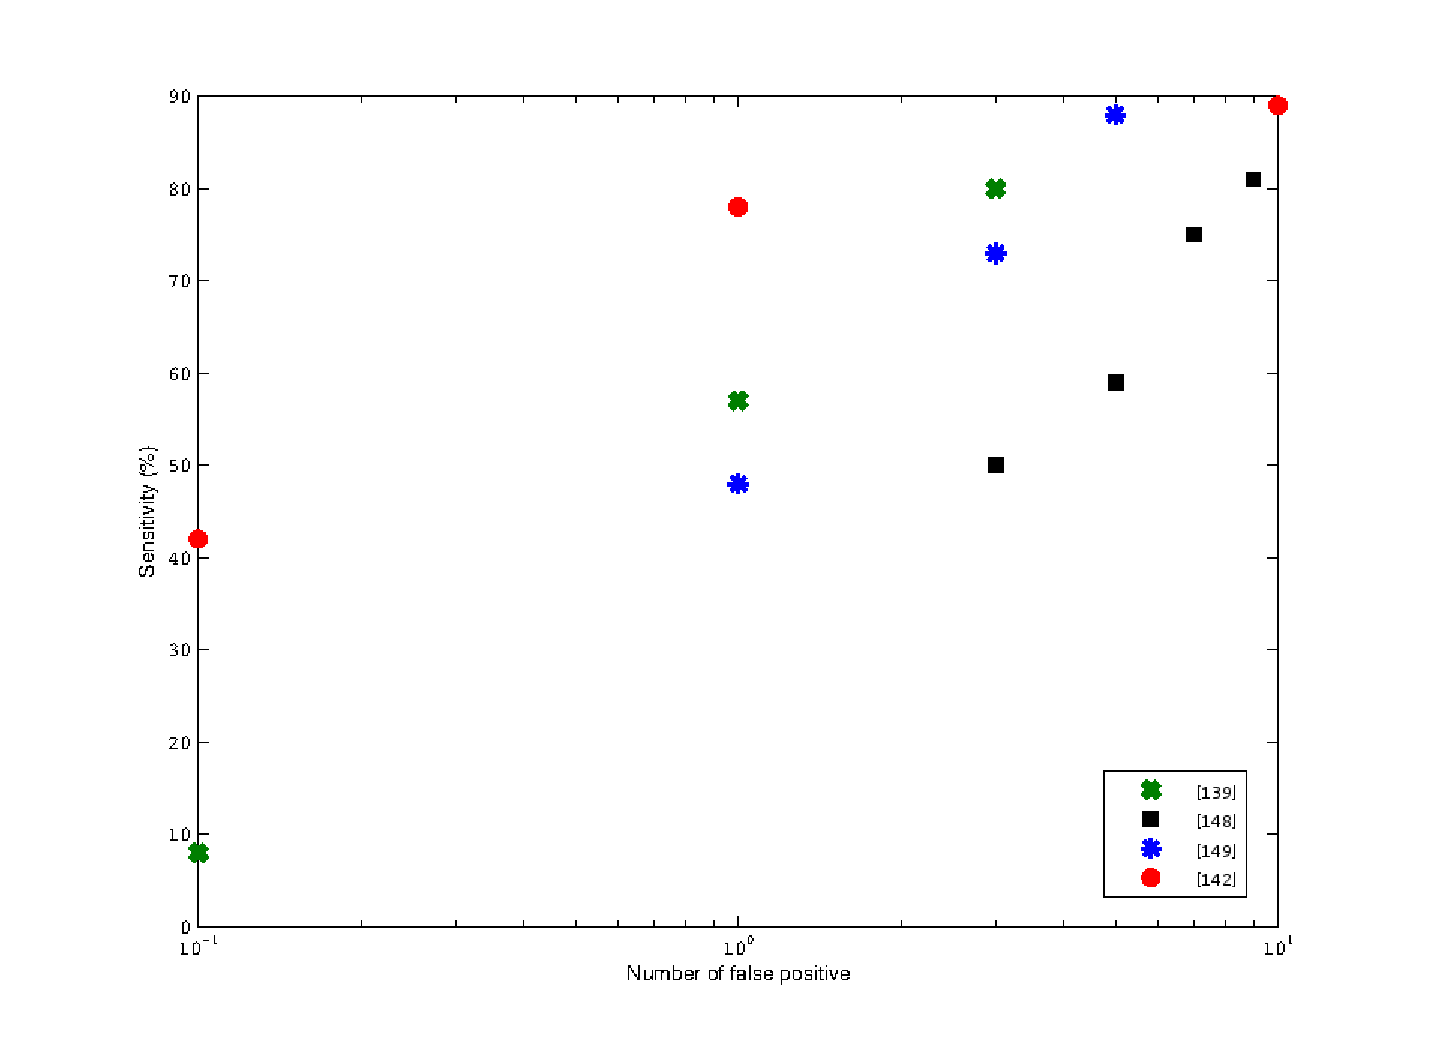
\includegraphics[width=.6\linewidth]{12_figures/figures/froc/froc.eps}
  \caption{Comparison in terms of \ac{froc} of the methods using data from 3.0 Tesla \ac{mri} scanner.}
  \label{fig:froc}
\end{figure}

%%% Local Variables: 
%%% mode: latex
%%% TeX-master: "../g_lemaitre_state_of_the_art"
%%% End: 
